\chapter{Clustering Retweets}
\markright{\thechapter \,\,\currentname \, - Philipp Kappus}
\label{chap:cluster_retweets}
Wie in Abschnitt \ref{sec:struktur-eines-tweets} beschrieben enthält ein \gls{Retweet} die Informationen des/der Nutzer*in der/die ihn veröffentlicht hat, sowie die Informationen des/der Nutzer*in der/die den Original-Tweet veröffentlicht hat. Eine Beziehung kann also zwischen diesen Beiden Nutzer*innen hergestellt werden. Außerdem kann durch die Anzahl an \glspl{Retweet} der Beziehung eine Gewichtung zugeschrieben werden. Durch Analyse aller \glspl{Retweet} kann so ein Netz von Beziehungen zwischen Nutzern*innen aufgebaut werden.
Werden in diesem Netz Nutzer*innen identifiziert, die sich häufig untereinander \glspl{retweetet} so können diese einer Gruppe zugeordnet werden. Im Folgenden soll der Prozess solche Gruppen zu finden, dargestellt und die Ergebnisse präsentiert werden.

\section{Daten vorbereiten}
\label{sec:daten-vorbereiten}
Zur Verarbeitung und Analyse der Daten wurde keine Datenbank verwendet sondern ausschließlich mit Dateioperationen und Ordnerstrukturen gearbeitet. Somit können die Daten in jeder beliebigen Art und Strukturierung abgelegt, Metainformationen hinzugefügt und jeder Schritt des Prozesses zwischengespeichert werden. 
Um die Tweets auf Beziehung zwischen Nutzer*innen zu schließen wurden folgende vorbereitende Schritte ausgeführt:
\begin{enumerate}
	\item \textbf{Daten aus \gls{S3 - Bucket} herunterladen}
	\item \textbf{Unrelevante Informationen filtern}\\  So wird ein übersichtliches Format erreicht und Speicherplatz gespart. Das resuliertende Tweet-Objekt entspricht der Beschreibung aus Abschnitt \ref{sec:struktur-eines-tweets}
	\item \textbf{Tweets in einer Ordnerstruktur nach Nutzer sortieren\\} Als eindeutige Identifikation wurde der in Abschnitt \ref{sec:struktur-eines-tweets} genannte Nutzername gewählt. Es ensteht folgende Ordnerstruktur: \\
	\dirtree{%
		.1 /.
		.2 Nutzer1.
		.3 Tweet1.json.
		.3 Tweet2.json.
		.2 Nutzer2.
		.3 Tweet1.json.
		.3 Tweet2.json.
		.3 Tweet3.json.
	}
	\item \textbf{Metadaten erstellen}\\
	Nun soll für jede*n Nutzer*in Metadaten erstellt werden, von wem und wie oft er von anderen Nutzer*innen \gls{geretweetet} wurde.
	Dafür werden alle Nutzer*innen und ihre Tweets analysiert; ist einer davon ein \gls{Retweet} eines andere*n Nutzer*in so wird das, zusammen mit der Anzahl, in den Metdaten desjenigen Nutzers, der \gls{geretweetet} wurde, vermerkt. 
	Für jeden Nutzer entstehen damit Metadaten der Form:
	\lstset{
		string=[s]{"}{"},
		stringstyle=\color{blue},
		comment=[l]{:},
		commentstyle=\color{black},
	}
	
	\begin{lstlisting}[caption={Metdaten des Nutzer: "`tagesschau"'}]
		{
			"i_was_retweeted_by": {
				"RSplettsto": 2,
				"Roxana50189220": 2,
				"RobbyTipps": 14,
				"RafaelOsswald": 2,
				"rbbinforadio": 16
			},
			"i_am_retweeting": {
				"tagesthemen": 6,
				"ARD_BaB": 3,
				"aktuelle_stunde": 1,
				"gudrun_engel": 1
			}
		}
	\end{lstlisting}
\end{enumerate}
Dieser Prozess besitzt eine Komplexität von $\mathcal{O}(n)$ mit $n$ = Gesamtanzahl an Tweets. 
\section{Influencer identifizieren}
\label{sec:influencer}
Bei der Untersuchung der Metadaten von März 2021, ist aufgefallen, dass 31,54\% aller \glspl{Retweet} auf die 100 meist geretweeteten Nutzer entfällt (0,04\%).
Genauer folgt die Verteilung einem inversen Potenzgesetz:
\begin{equation}
	\begin{aligned}
		N_{retweets} = b*x^{-m}\\
		m = 0.65\\
		b = 39,215
	\end{aligned}
\end{equation}
wobei $x$ der Rang, $m$ die Steigung und $b$ der Skalierungsfaktor oder die Anzahl der Retweets des Influencers an Rang 0 ist.\\
\begin{figure}[h!]
	\centering
	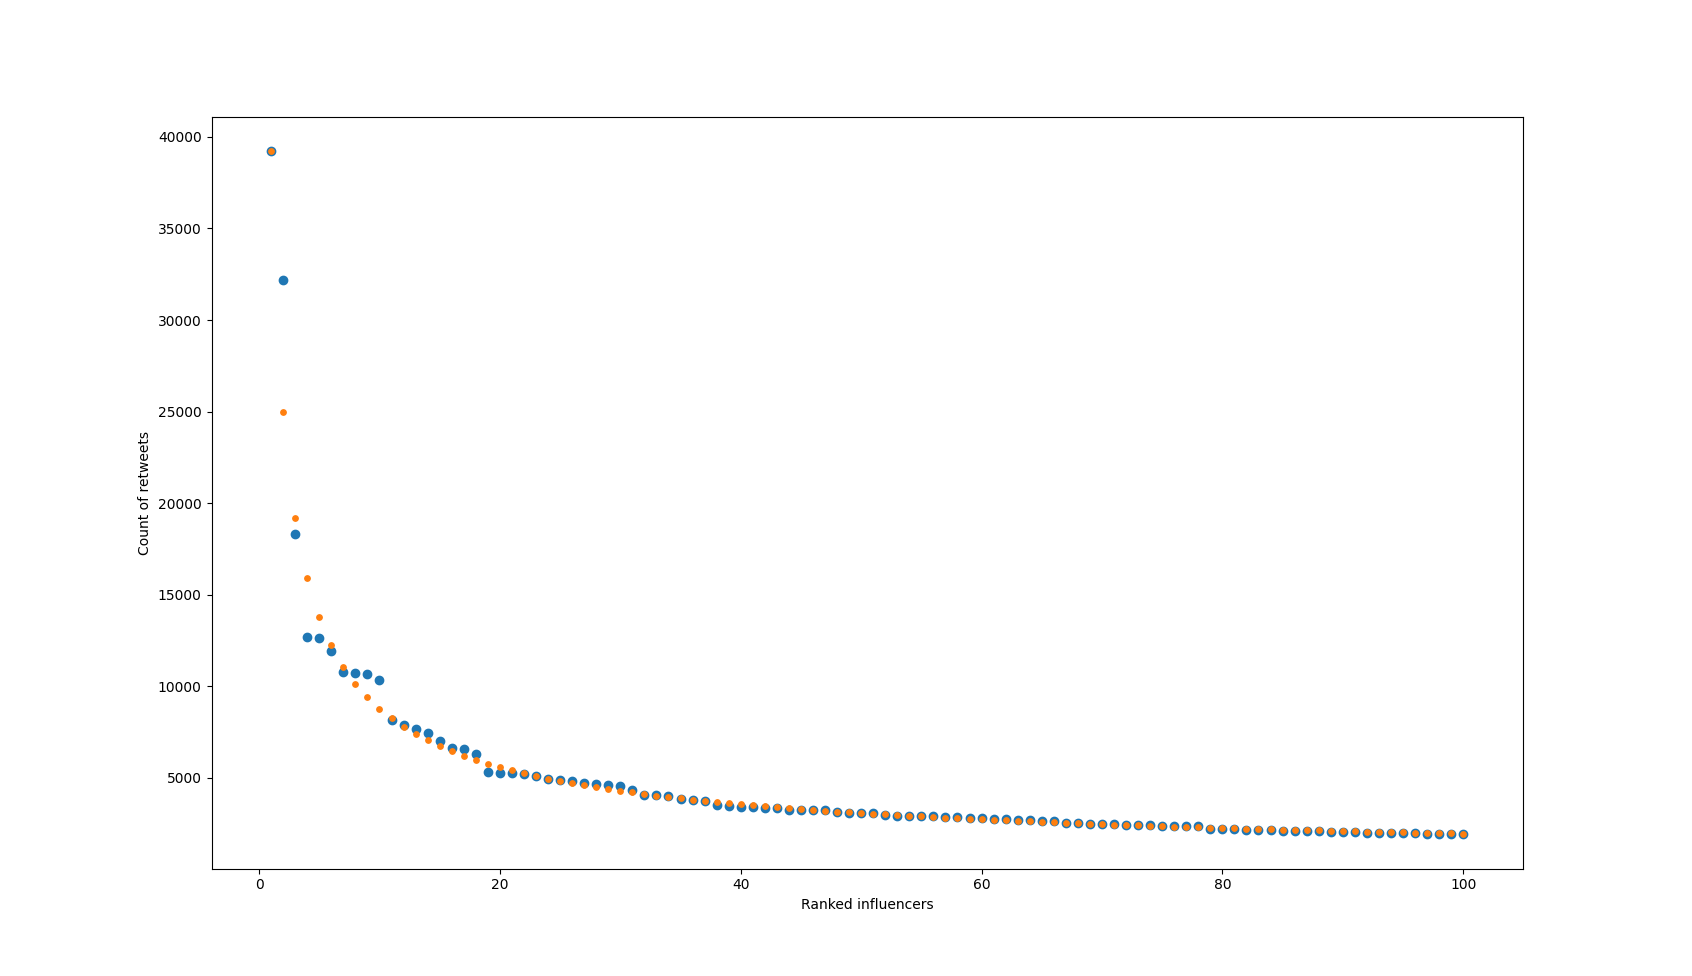
\includegraphics[width=0.8\linewidth]{images/power-law}
	\caption{Verteilung der Anzahl an \glspl{Retweet} (blau) und das inverse Potenzgesetz (orange)}
	\label{fig:tweetverteilung}
\end{figure}
Daraus wurde der Schluss gezogen, dass Beziehungen zwischen "`kleineren"' Nutzer*innen vernachlässigbar sind und nur Verbindungen zu den 100 meist \glspl{geretweetet} Nutzer*innen von Bedeutung sind. Diese werden im Folgenden "`Influencer"' genannt. Auch kann davon ausgegangen werden, dass Beziehung zwischen "`kleineren Nutzern"'  repräsentiert sind, da zwei Nutzer*innen die sich gegenseitig \glspl{retweetet}, wahrscheinlich auch eine Beziehung zur gleichen Influencer haben. 
Diese Methodik vermindert die Anzahl an Verbindungen und führt zu einer effizienteren Verarbeitung der Daten sowie später zu einem übersichtlicheren Graphen (siehe Abschnitt \ref{sec:aggregieren})
Die Anzahl an Influencern ist wählbar und führt zu verschiedenen Ergebnisse, allerdings hat sich 100 als ein passender Parameter herausgestellt. Dieser Sachverhalt wird in Abschnitt näher diskutiert.

\section{Nutzergruppen aggregieren}
\label{sec:aggregieren}
 Influencer $I$ und Nutzer*innen $N$ können als Knoten $K = I \cup N$,  Beziehungen als gewichtete Kanten $E$ eines Graphen $G = (K,E)$ betrachtet werden.
Dieser kann als ungerichtet definiert werden, da Kanten immer zu einem Influencer zeigen.
$E$ ist hierbei eine Menge an Paaren der Form ($i\in I$,$n\in  N$,$g$) wobei $g$ die Anzahl der \gls{Retweet} darstellt. 
Dieser Graph kann visualisiert werden. Genutzt wurde dafür \gls{Python3}, \gls{Matplotlib} und eine NEATO Implementierung als \gls{Layoutalgorithmus} (siehe \cite{neato}).
\begin{figure}[h]
	\centering
	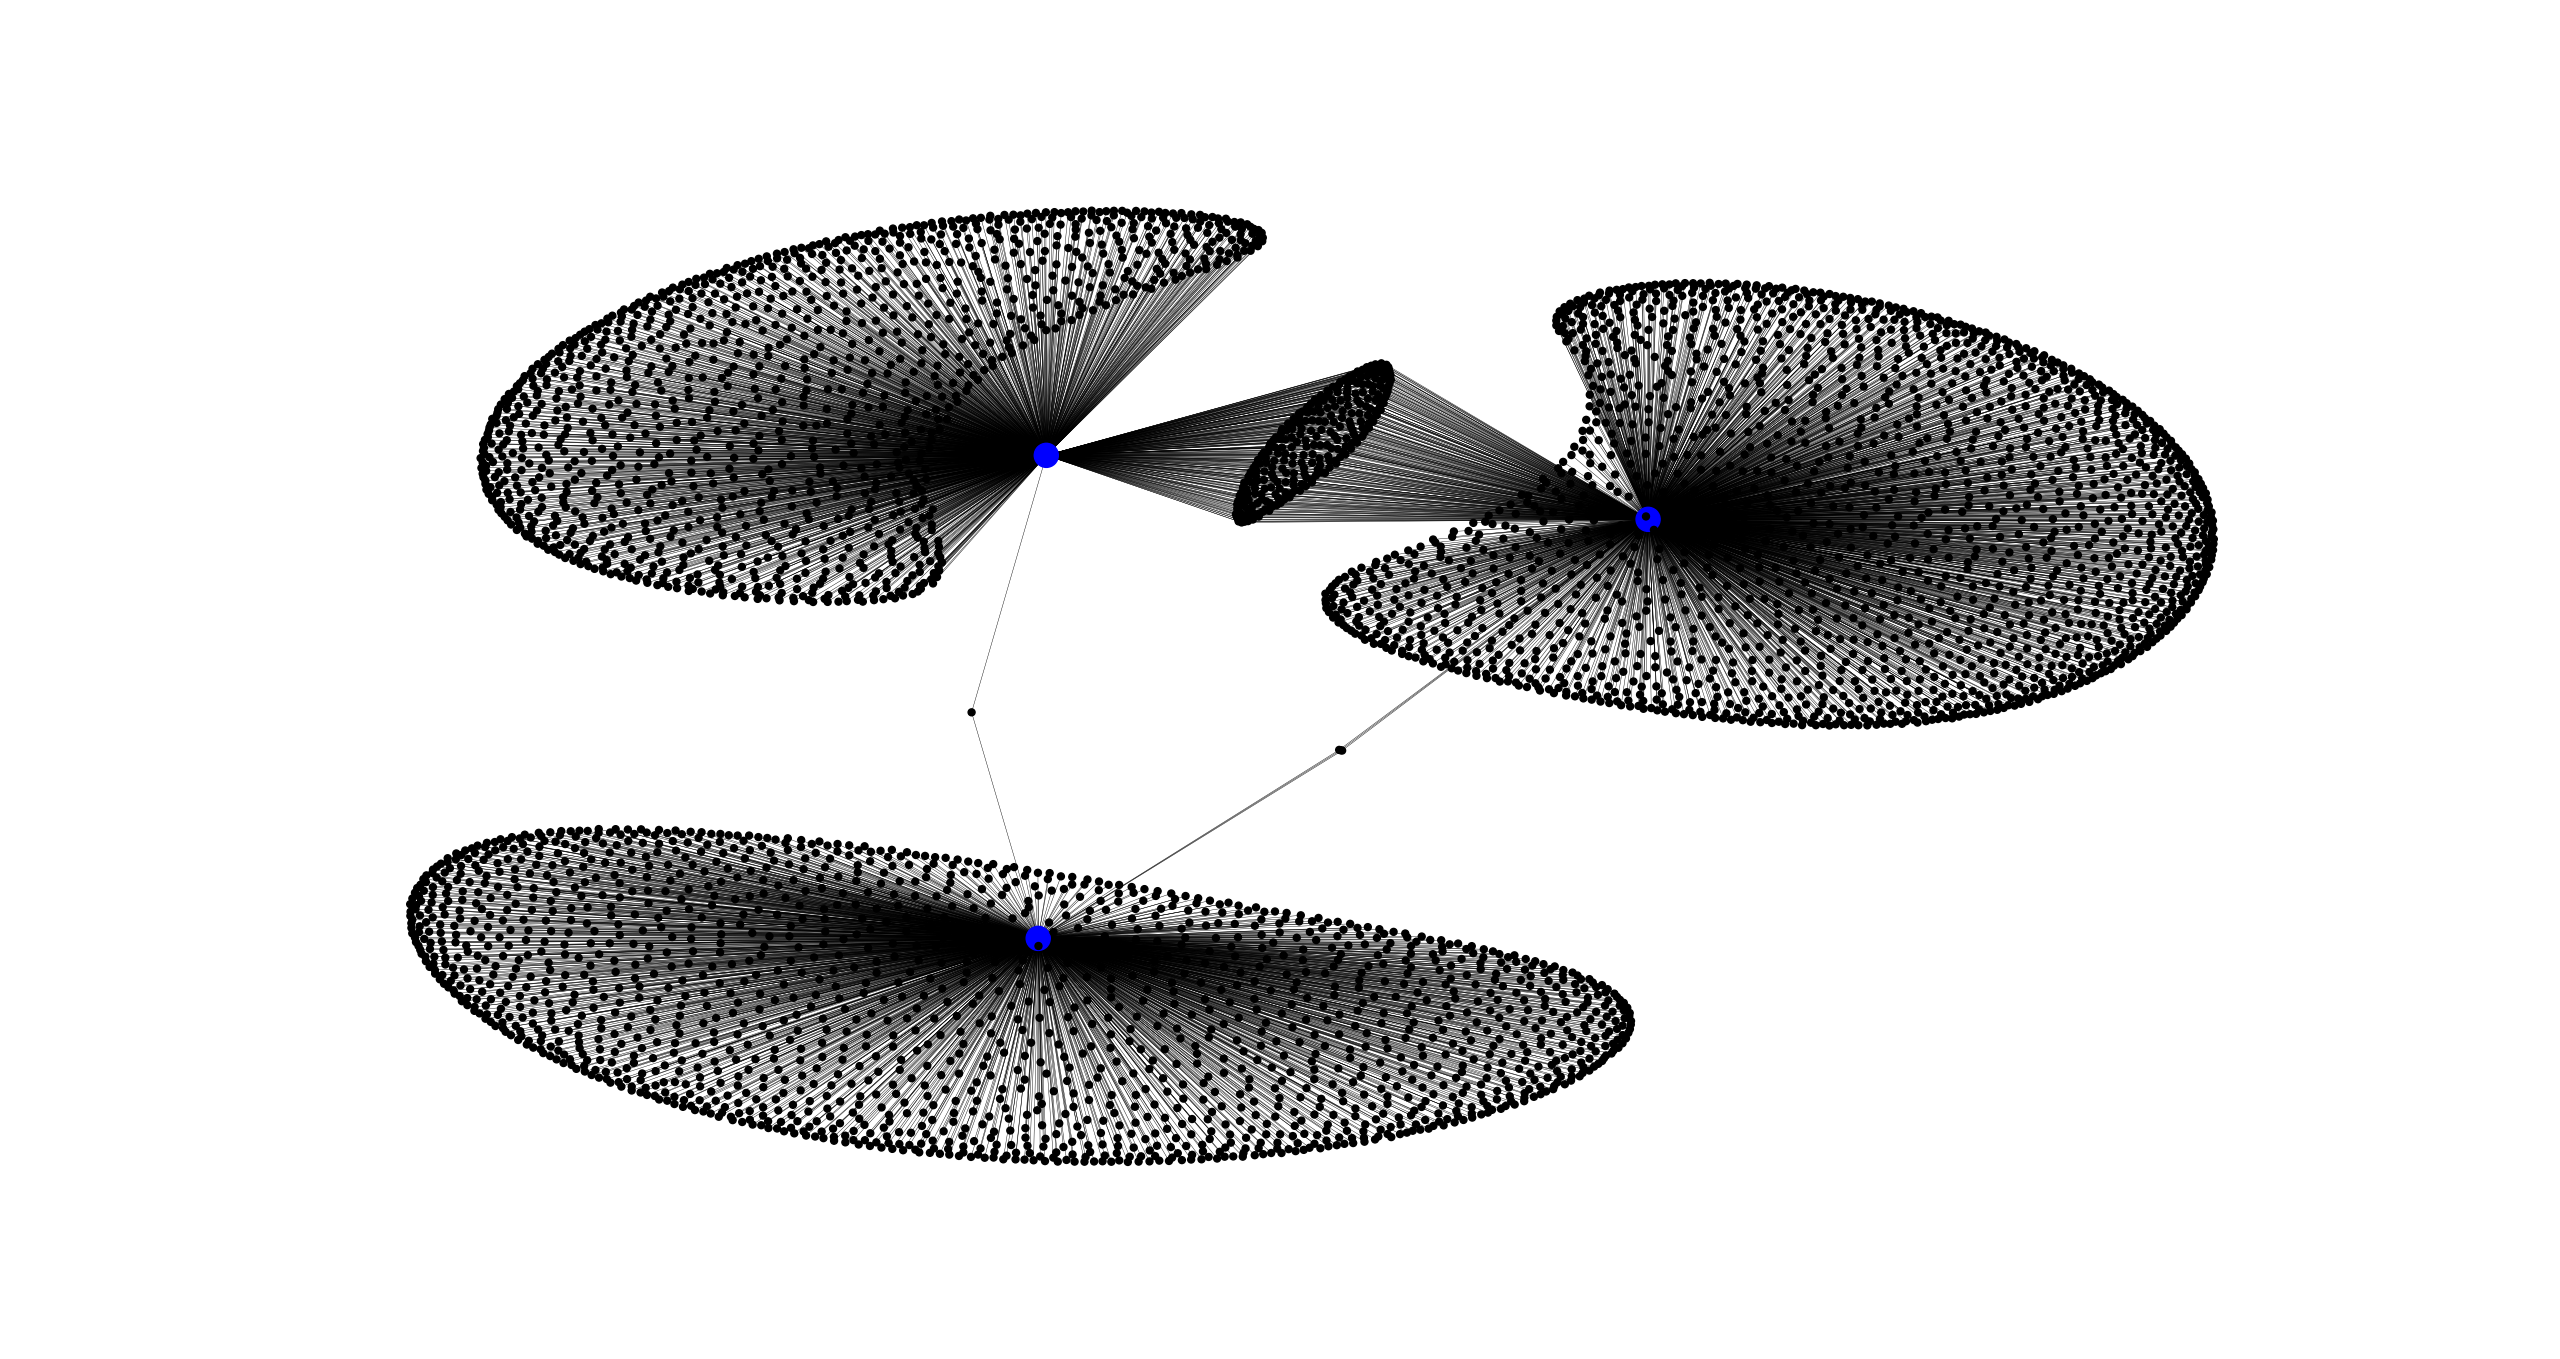
\includegraphics[width=\linewidth]{images/GraphNoAggregation}
	\caption{Graph mit drei Influencern (blau)}
	\label{fig:graphnoaggregation}
\end{figure}

Abbildung \ref{fig:graphnoaggregation} zeigt einen solchen Graph mit Daten aus 4 Tagen, den drei Influencern in blau (Karl\_Lauterbach, reitschuster, Volksverpetzer) und allen Nutzer*innen die diese \gls{geretweetet} haben in schwarz. Die Berechnung dieses Layout braucht auf einen handelsüblichen PC mit Linux 35,6 Sekunden. 
Mit Daten von mehr als 4 Tagen oder mit mehr als 3 Influencern explodiert die Berechnungszeit. 
Offensichtlich erkennbar ist, dass es  für jede Influencer eine Menge an Nutzer*innen $N_{i^x}$ gibt, die nur diese Influencer \gls{geretweetet} haben.
Analog dazu gibt es eine Menge an Nutzer*innen $N_{i^1i^2}$ die sowohl Influencer $i^1$ und Influencer $i^2$ retweeten. 
Diese Mengen können als "`Superknoten"' betrachtet werden, der alle Nutzer*innen repräsentiert, die z.B. sowohl $i^1$ als auch $i^2$ \gls{geretweetet} haben.
Es gilt also für einen Superknoten $s$:
 \begin{equation}
s_{i^n\,..\,i^m} = \{n\in N|\forall e(n,i^n\,..\,i^m)\in E\}
\end{equation}
Die Gewichte $g$ der Kanten werden aufaddiert. 
Damit lässt sich der Graph auf maximal
\begin{equation}
|K| = |S| + |I| = \sum_{n=1}^{|I|} \binom{|I|}{n} + |I| = 2^{|I|} - 1 + |I|
\end{equation}
Knoten beschränken (mit $|S|$ der Menge aller möglichen Superknoten).
\begin{figure}[h]
	\centering
	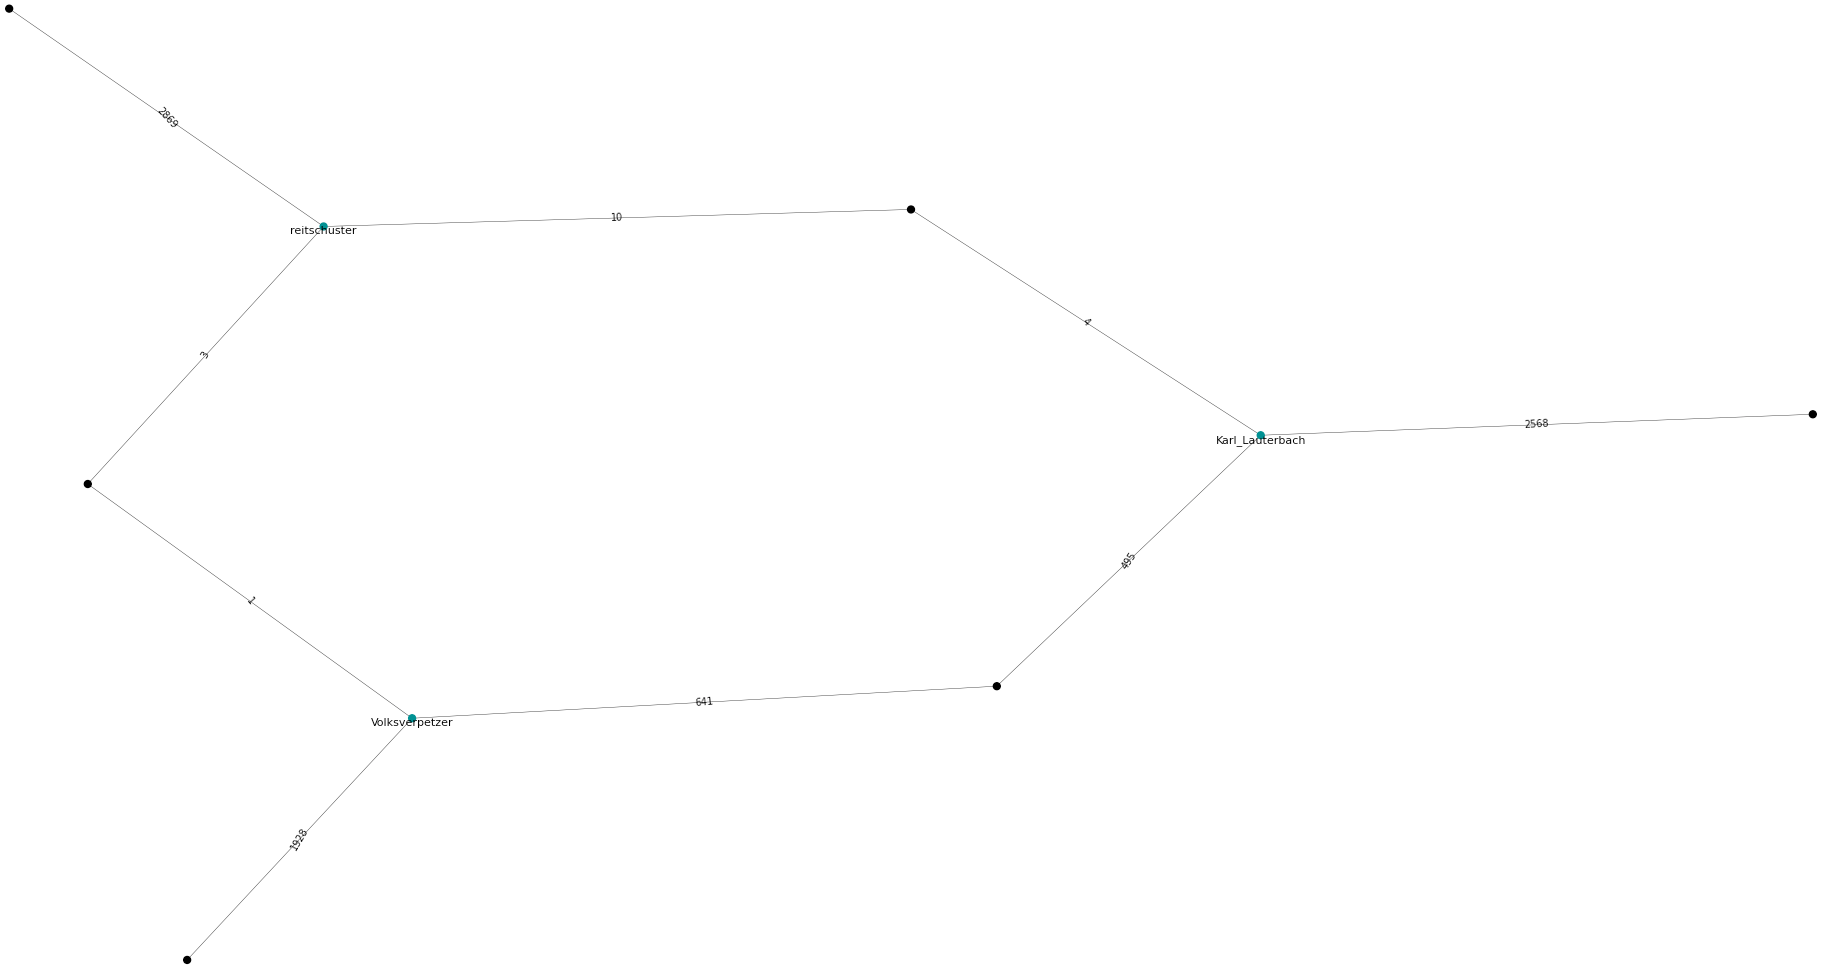
\includegraphics[width=0.7\linewidth]{images/GraphNoThreshold}
	\caption{Graph mit aggregierten Superknoten}
	\label{fig:graphnothreshold}
\end{figure}
Abbildung \ref{fig:graphnothreshold} zeigt den selben Graph wie \ref{fig:graphnoaggregation} mit zu Superknoten aggregierten Nutzern.
Die Berechnung des Layout konnte dadurch auf 0.16 Sekunden reduziert werden.
Auch dieser Prozess besitzt eine Komplexität von $\mathcal{O}(n)$ mit $n$ = Gesamtanzahl an Nutzern. 
\section{Kanten filtern}
\label{sec:kanten-filtern}
Wie in Formel 5.2 und Abbildung \ref{fig:superknotenentwicklung} zu sehen, steigt die Anzahl an möglichen Superknoten expotentiell mit steigender Zahl an Influencern.
\begin{figure}[h]
	\centering
	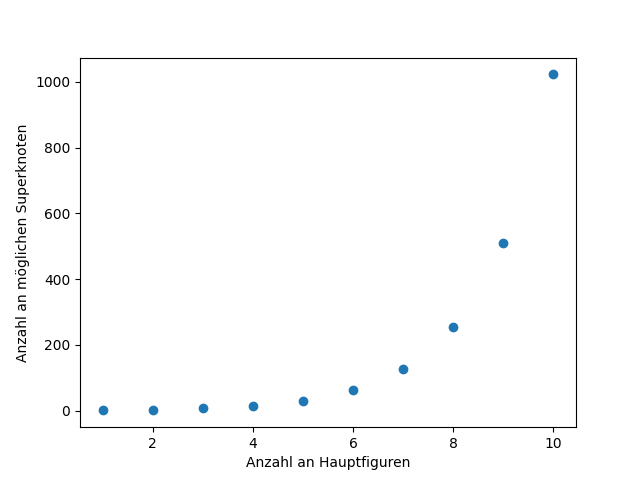
\includegraphics[width=0.7\linewidth]{images/Superknotenentwicklung}
	\caption{Entwicklung der möglichen Superknoten mit der Anzahl an Influencern}
	\label{fig:superknotenentwicklung}
\end{figure}
Bei $|I| = 100$ könnten bis zu $1.26*10^{30}$ Superknoten existieren. Das ist für jegliche Berechnung oder Darstellung unpraktikabel.
Deshalb wird auch hier eine Komplexitätsverringerung durch Filtern unrelevanter Information vorgenommen indem alle Kanten von einem Superknoten zu einer Influencer gelöscht werden, die unter einem Schwellwert liegen. 
Es wird davon ausgegangen, dass  bei einem niedrigen Kantengewicht die Nutzer*innen nur eine schwache Beziehung zu dem entsprechenden Influencer haben und diese damit für eine spätere Gruppierung irrelavant ist. 
Wie dieser Schwellenwert festgelegt wird, wird in Abschnitt \ref{sec:clutering} diskutiert. 
Es gilt also mit dem Schwellwert $T$: \begin{equation}
	E_{gefiltert} = \{(s,i,g)\in E|g>T\}
\end{equation}

Wurde eine Kante (z.B. $(s,i^3)$) von einem Superknoten $s_{i^1i^2i^3}$ gelöscht, so ändert sich dieser zu $s_{i^1i^2}$. Nun ist es allerdings möglich, dass der Knoten $s_{i^1i^2}$ bereits existiert, was zu einer Verdopplung der eigentlich gleichen Kante führt. Dies kann vermieden werden indem nach dem Löschen einer Kante überprüft wird ob der so enstandene Superknoten bereits existiert. Falls ja, werden diese zusammengeführt indem die jeweiligen Kantengewichte addiert werden.
Des Weiteren werden diejenigen Superknoten gelöscht, die Nutzer repräsentierten, die nur eine Influencer \gls{geretweetet} haben, da sie für eine Eingruppierung anhand von Beziehung keine Relevanz haben.
Dieser Prozess besitzt eine Komplexität von $\mathcal{O}(n^2)$ mit $n$ = Gesamtanzahl der Superknoten, da im schlechtesten Fall für jeden veränderten Knoten, dieser mit alle bereits bestehenden Knoten auf Gleichheit überprüft werden muss.
\section{Kantengewichte normalisieren}
Wie in Abschnitt \ref{sec:influencer} beschrieben folgt die Verteilung der Retweets auf die Influencer einem inversen Potenzgesetz.
Der Natur eines inversen Potenzgesetzes folgend, haben die niedrigen Ränge eine deutlich höhere Anzahl von Retweets, was es schwierig macht, einen Schwellenwert zu finden, der einerseits die Komplexität in Bezug auf Verbindungen mit dem niedrigrangigen Influencer minimiert, aber trotzdem Gruppen erhält, die aus höherrangigen Influencern bestehen.
Um diesem Problem entgegenzuwirken, werden Kantengewichte von Einflussfaktoren mit dem Zehner logarithmus des Rangs des jeweiligen Influencers multipliziert, bevor der Schwellenwert angewendet wird.
Dies normalisiert die Retweets nicht vollständig, da ansonsten Retweets von höherrangigen Influencern überbewerten würden.
Trotzdem verringert es die Dominanz von niederrangigen Influencern.
\begin{figure}[h!]
	\centering
	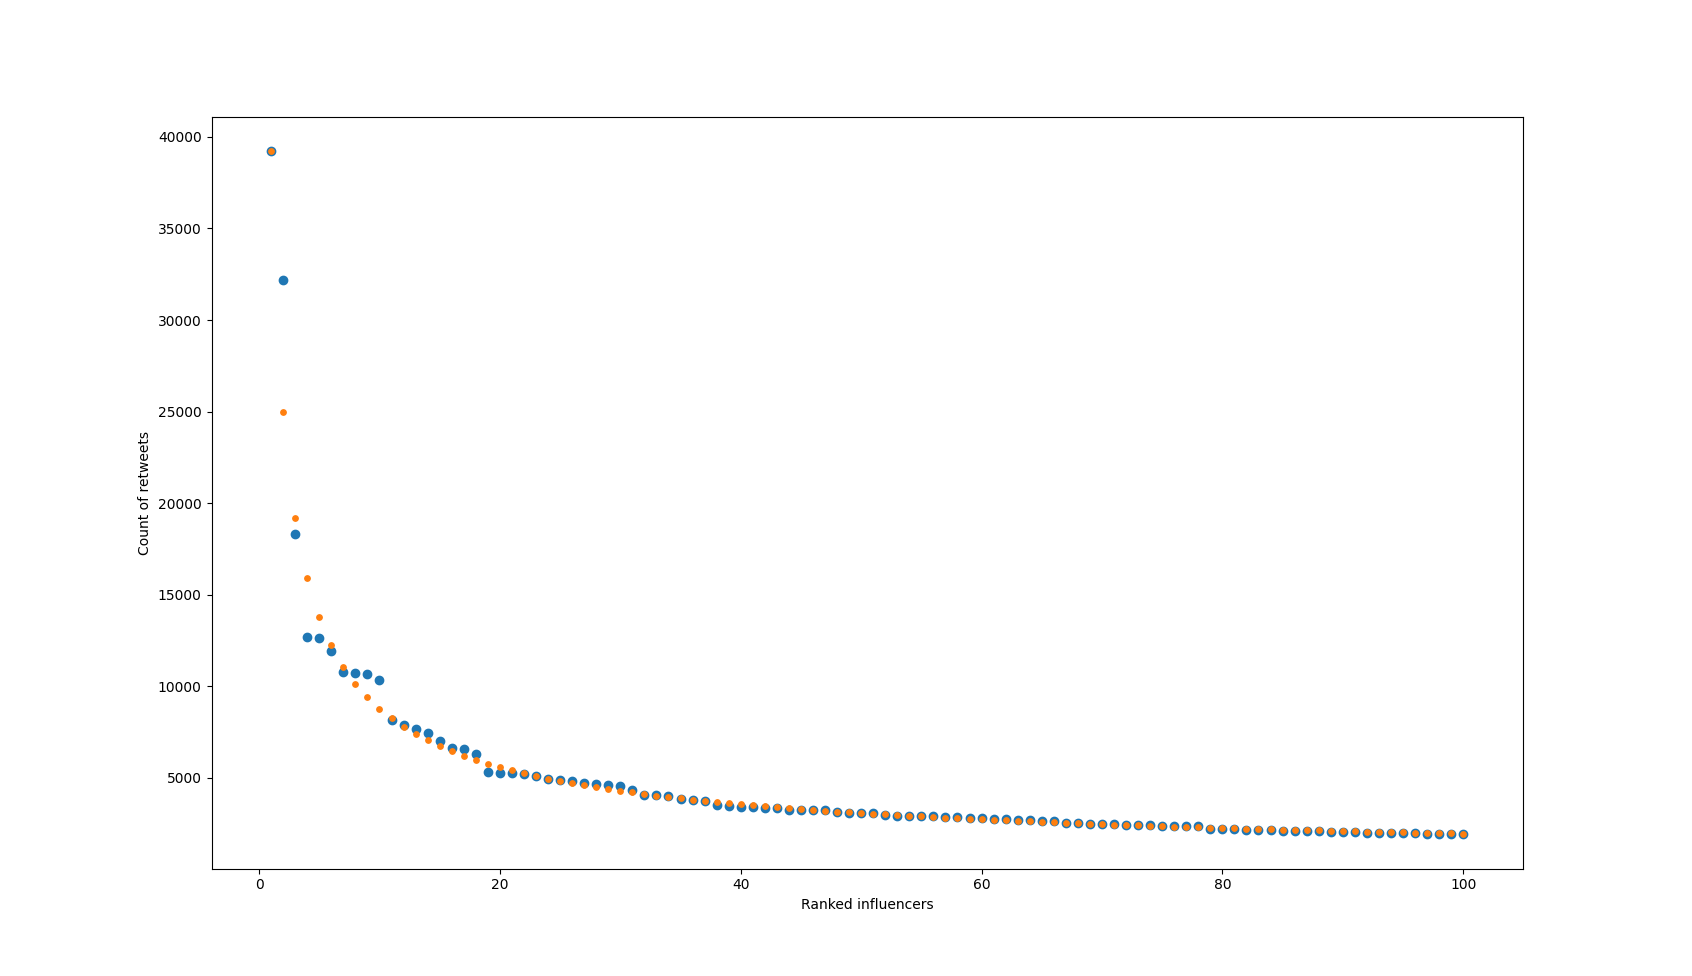
\includegraphics[width=\linewidth]{images/power-law}
	\caption{The distribution of retweets (blue) and the power-law from equation 4(orange)}
	\label{fig:power-law}
\end{figure}
\section{Clustering}
\label{sec:clutering}
Das Ergebnis aller bisherigen Prozessschritte mit den Daten von März 2021 (2,955,282 Tweets, 260,954 Nutzer), 100 Influencern und einem Schwellenwert von 61 ist in Abbildung \ref{fig:noclusters} zu sehen und wurde innerhalb von 2 Stunden und 58 Minuten berechnet. 
\begin{figure}[h!]
	\centering
	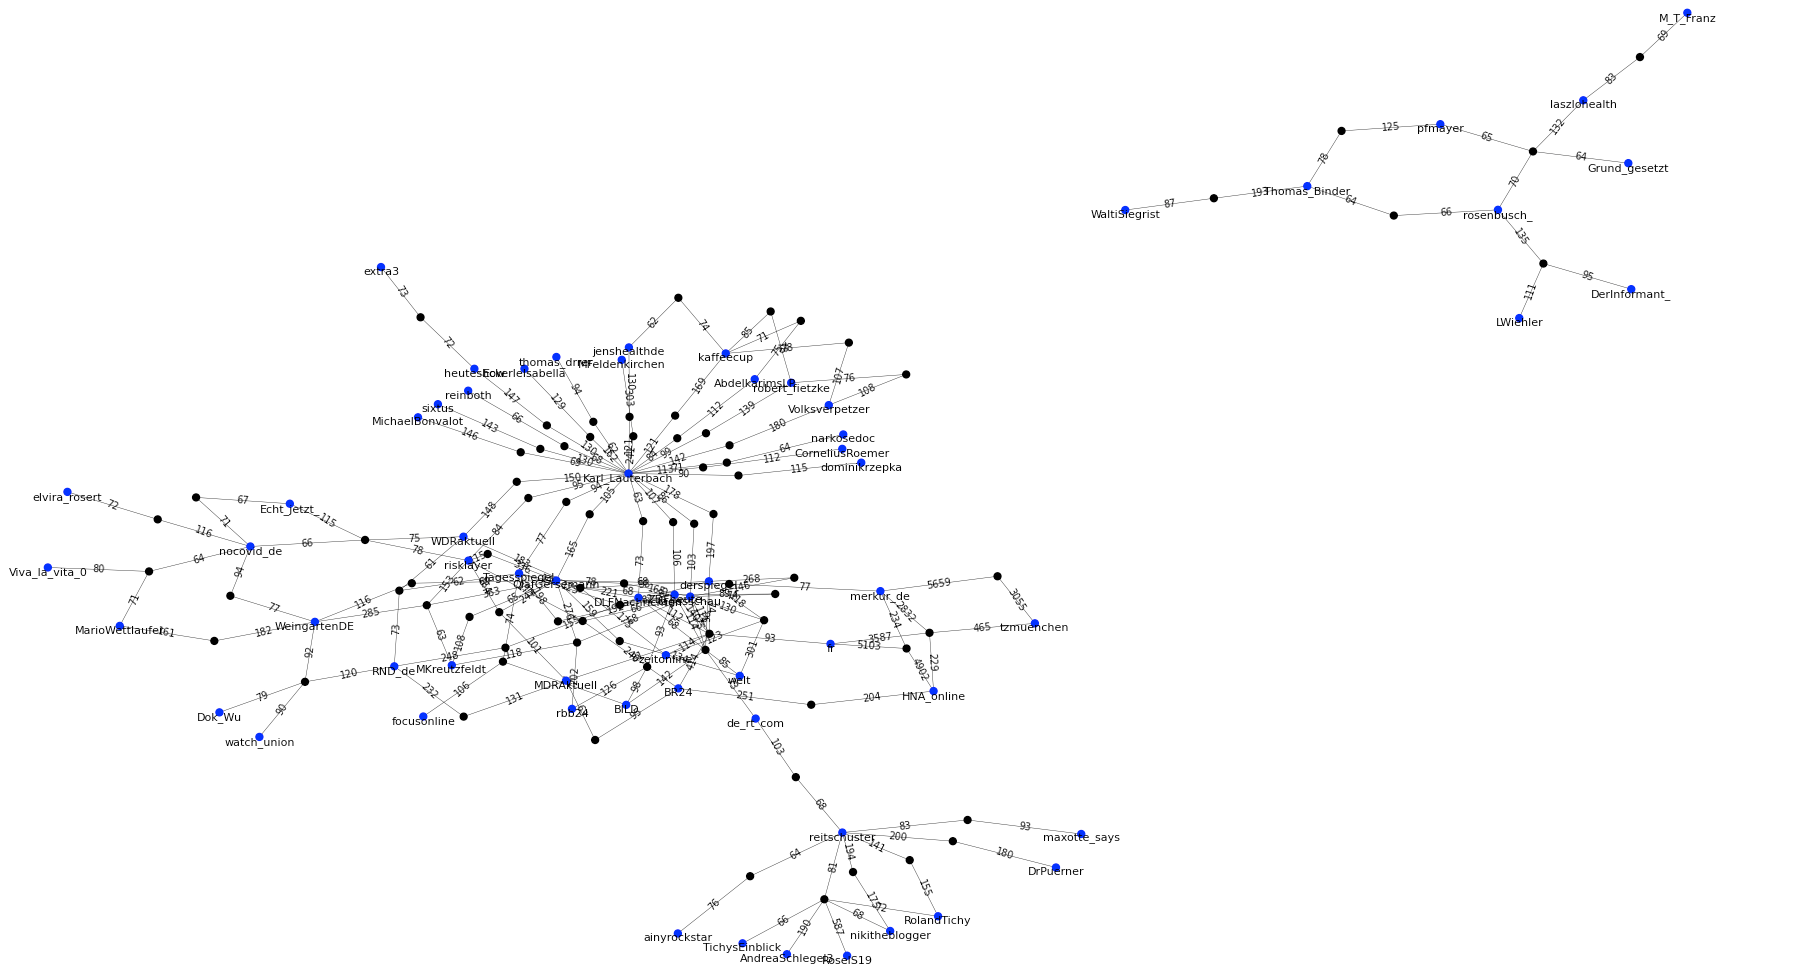
\includegraphics[width=\linewidth]{images/NoClusters}
	\caption{Ergebnisgraph März 2021}
	\label{fig:noclusters}
\end{figure}
Als Mensch kann man ein  großes zentrales \gls{Cluster}, eins das mit diesem verbunden ist (unten) und ein seperates \gls{Cluster} (oben links) erkennen. 
Im Folgenden wird dargelegt, wie diese \gls{Cluster} automatisch erkannt werden.
Zu einem \gls{Cluster} können in diesem Kontext alle Knoten gezählt werden, die dicht miteinander verbunden ist; das heißt sie stehen über einige weitere Knoten in Beziehnung.
Da eine Anzahl an \gls{Cluster} vorher nicht festgelegt werden kann und es kein geometrischen Raum gibt (nur die Verbindungen zählen, die Positionen der Punkte irrelevant) wurde sich hier für eine abgewandelte Form des DBSCAN - Algorithmus entschieden (siehe \cite{dbscan}).
Als Knoten werden nur Influencern betrachtet da die Superknoten nur die Verbindung zu weiteren Influencern darstellen. 
Die Nachbar eines Influencer sind alle Influencern die mit dem Ausgangsinfluencer über ein Superknoten verbunden sind (siehe Abbildung \ref{fig:dbscan-neighbours})
\begin{figure}
	\centering
	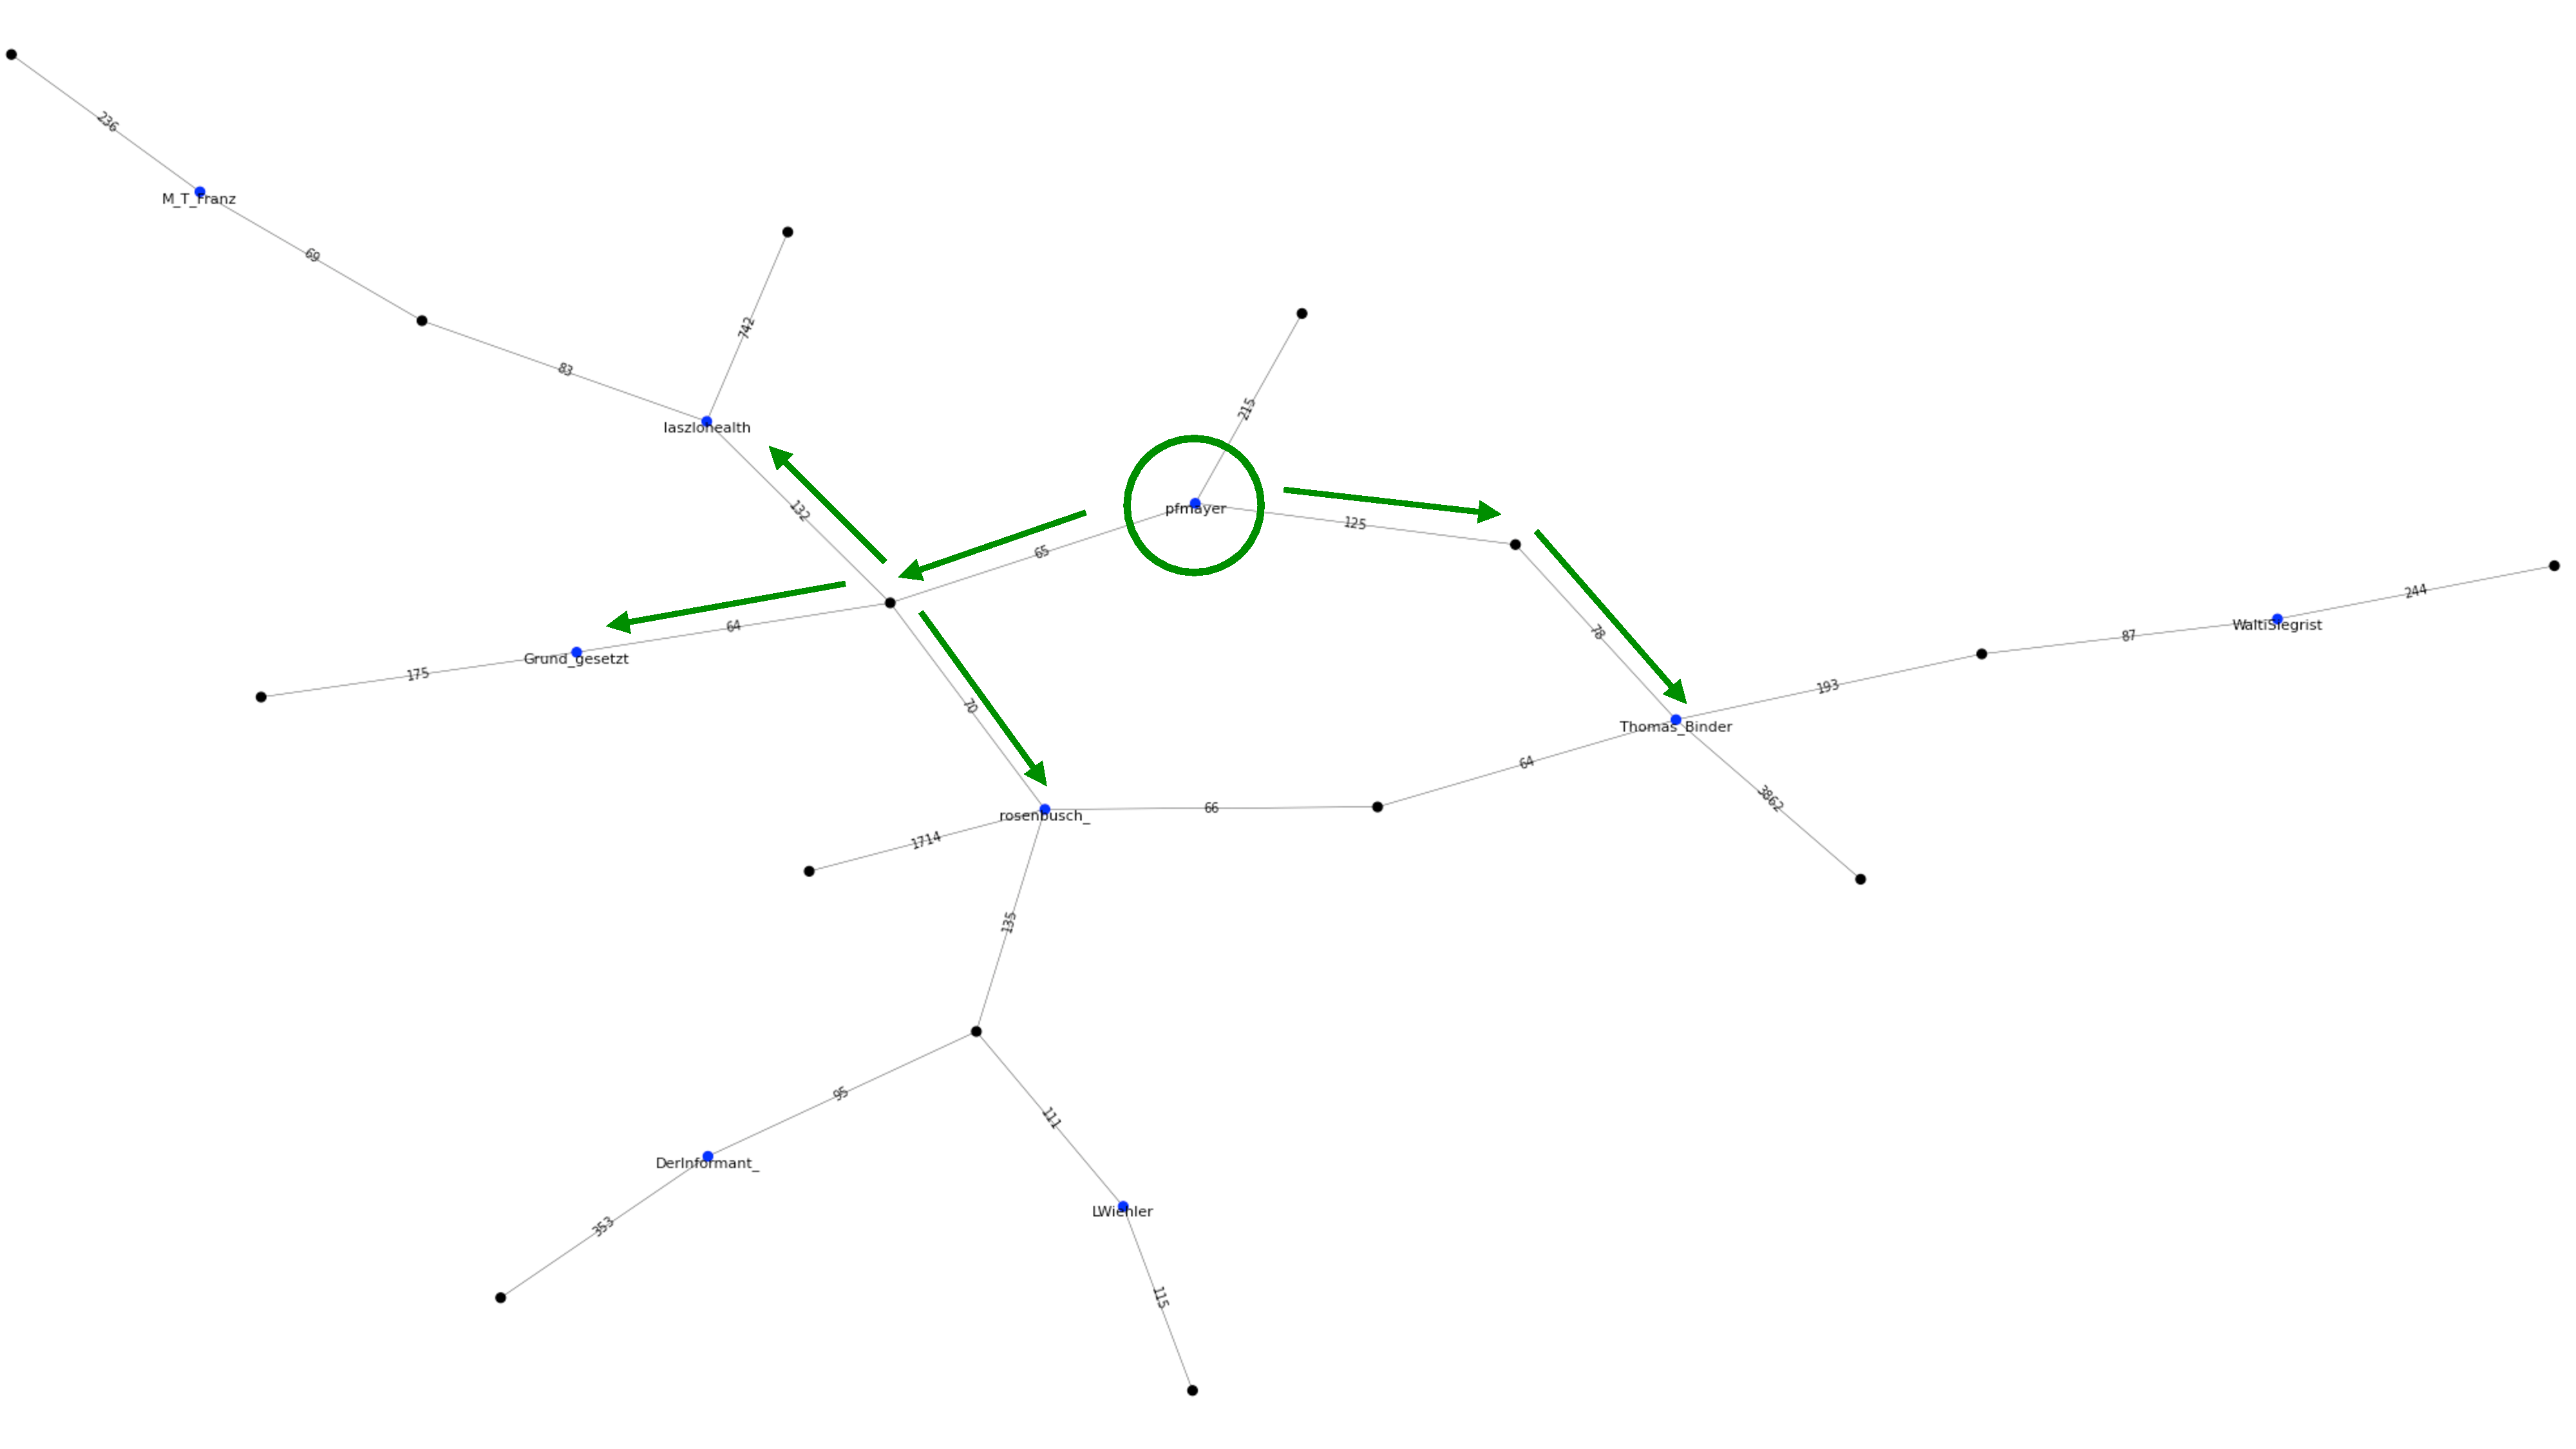
\includegraphics[width=0.7\linewidth]{images/DBSCAN-neighbours}
	\caption{Nachbarn eines Influencer über verbundene Superknoten}
	\label{fig:dbscan-neighbours}
\end{figure}
Eine Mindestdistanz $\epsilon$ wird nicht benötigt, da alle Verbindungen die dadurch nicht gezählt würden, bereits durch den in Abschnitt \ref{sec:kanten-filtern} definierten Schwellwert aussortiert wurden.
Da mit diesem Ansatz jede Verbindung zu eines weiteren Influencer als Nachbar in den DBSCAN eingeht, werden \gls{Cluster} die nur leicht verbunden sind (wie in Abbildung \ref{fig:noclusters} das Zentrale und das unten Positionierte) als ein \gls{Cluster} definiert. 
Um hier eine Trennung zu schaffen, werden nur Knoten als Nachbarn gezählt die noch nicht dem aktuellen \gls{Cluster} zugeordnet wurden wie in Listing \ref{lst:neighborfunction}.
\begin{lstlisting}[language=Python,caption={Abwandlung der DBSCAN Nachbarfunktion},label={lst:neighborfunction}]
	def getNeighbors(node):
		all_neighbors = []
		supernodes = G.neighbors(node_name)
		for supernode in supernodes:
			real_neighbors = G.neighbors(supernode)
			for real_neigbor in real_neighbors:
				#Dieser Knoten wurde schon erreicht oder ist schon im aktuellen Cluster
				if(real_neigbor in cluster_nodes or neighbor_name in all_neighbors):
					continue
			all_neighbors.append(real_neighbor)
		return all_neighbors
\end{lstlisting}
Die Mindestanzahl an Nachbar damit ein Knoten zum Kernknoten wird, ist wählbar, allerdings hat sich ein Wert von 2 bewährt. Diese Wahl wird in Abschnitt diskutiert.
Auf den oben vorgestellten Datensatz angewendet, braucht das Berechnen der \gls{Cluster} 2,3 Minuten und liefert das in Abbildung \ref{fig:clustersscreenshot} dargestellte Ergebnis.
\begin{figure}[h!]
	\centering
	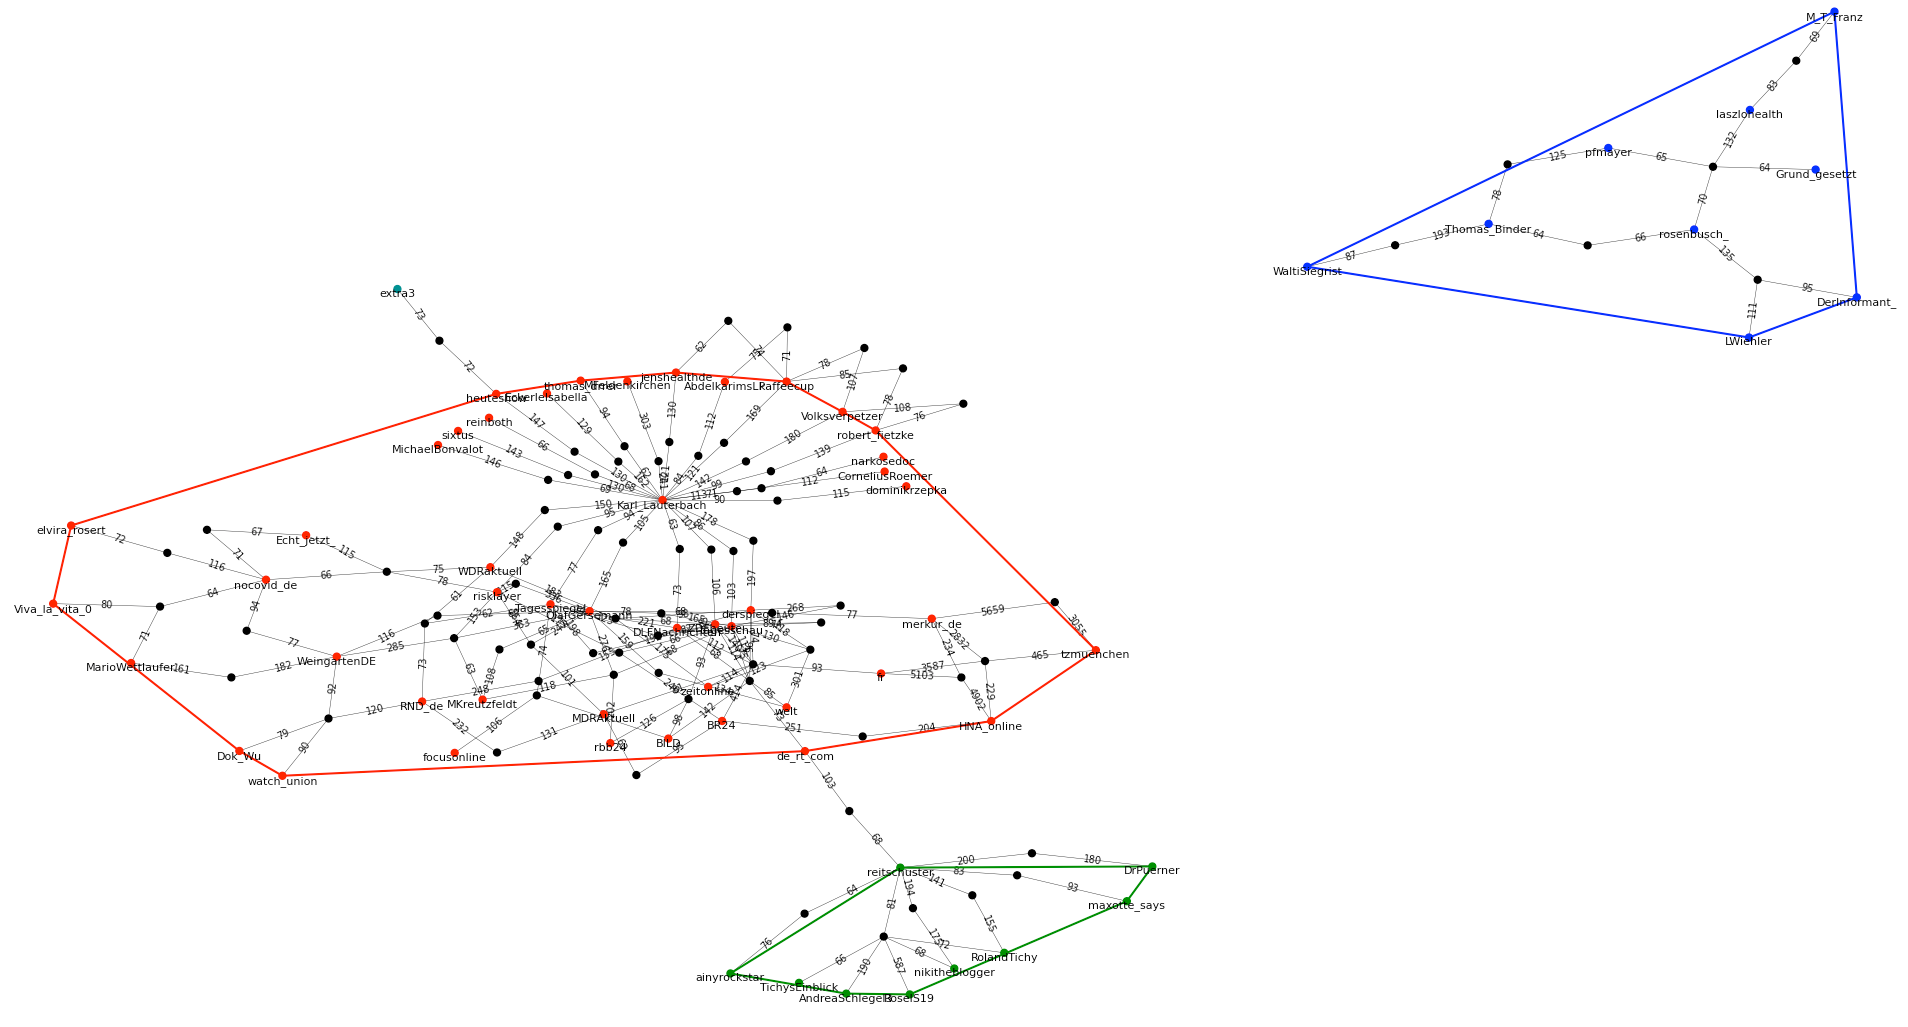
\includegraphics[width=\linewidth]{images/Clusters_screenshot}
	\caption{Graph mit Markierungen um die gefundenen \gls{Cluster}}
	\label{fig:clustersscreenshot}
\end{figure}

\section{Einblick in die Cluster}
\label{sec:einblick}
Um die anfängliche Frage zu beantworten, ob Gruppierungen von Menschen mit ähnlicher Sichtweise auf die Covid-19 Pandemie und die dazugehörigen Regelungen identifizert werden können, soll nun ein kurzer Überblick über die Charaktere der einzelnen Cluster gegeben werden. Das gelb markierte Hauptcluster besteht aus öffentlich-rechtlichen und privaten Nachrichtenagenturen wie "`ZDF"', `"tagesschau"', "`derspiegel"' oder "`BILD"' sowie dem am häufigsten \gls{geretweetet} Nutzer im Datensatz: "`Karl\_Lauterbach"', der, aufgrund seines Hintergrunds in der Sozialdemokratischen Partei (SPD) und als Mediziner, in der öffentlichen Debatte über die Pandemie eine präsente Figur ist.\\ \newline
Einige Influencer aus dem grünen Cluster sind: "`maxotte\_says"' (Max Otte) ehemaliger Vorsitzender der "`Werteunion"', eine Fraktion innerhalb der Christlich Demokratischen Union (CDU), bekannt dafür, konservativere Positionen zu vertreten, "`ainyrockstar"' eine rechter Journalistin \cite{schunke} und "`RolandTichy"' ehemaliger Herausgeber von "`Impuls"' und "`Euro"'.\\ \newline
Ein Blick in das obere rechte, orangefarbene Cluster:
"`rosenbusch\_"' (Henning Rosenbusch) ist ein unabhängiger Journalist, der sich für den "`Schweden-Weg"' einsetzt,
"`laszlohealth"' (unbekannt) mit einem gepinnten Tweet: \textit{"`Corona ist eine abartige Mischung aus Glaubens- \& Polit-Krieg mit allen Mitteln geworden. Die Maske das Symbol der Zugehörigkeit. PCR-Massen-Testung die Waffe. Sachlichkeit, Meinungsfreiheit, normalen Umgang gibt es nicht mehr."'}\cite{laszlo} und "`Thomas\_Binder"', dessen Account gesperrt wurde, ist ein schweizer Arzt, der eine Anti-Regulierungs-Position vertritt und verhaftet und in die Psychiatrie eingeliefert wurde wegen mutmaßlicher Drohungen gegen Politiker.\cite{Thomas}.
\section{Rückschluss auf Nutzer*innen}
Um nun nicht nur die Influencer eines Cluster sondern auch die Nutzer*innen, die diese geretweetet haben zu indetifizieren, wurde der Prozessschritt des Aggregierens (Abschnitt \ref{sec:aggregieren}) erweitern, sodass für jeden Supernutzer gespeichert wird, welche Nutzer ihn ausmachen.
Wurden nun die Cluster erstellt, können diesem Cluster auch alle Supernutzer zugeordnet werden, die mindestens eine Verbindungen zu einem Influencer aus diesem Cluster besitzen.
Aus den zugehörigen Supernutzer können nun auch alle "`normalen"' Nutzer*innen des Cluster extrahiert werden.
\section{Bestimmung der Themen innerhalb der Cluster}
\label{sec:topics}
Während in Kapitel \ref{sec:einblick} die Cluster anhand einzelne Individuen analysiert und damit in einen thematischen Zusammenhang gebracht wurden, soll im folgenden Anhand einer Wortanalyse das Thema innerhalb der Cluster bestimmt werden.
\begin{figure}[h]
	\centering
	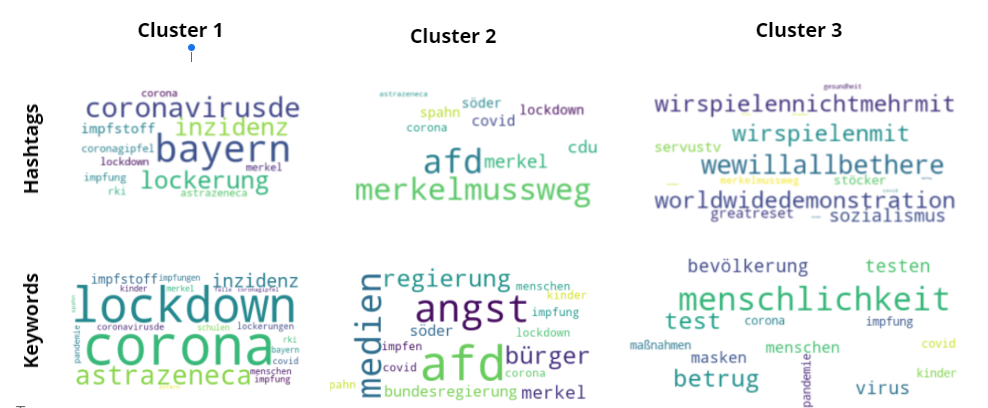
\includegraphics[width=\linewidth]{images/cluster_topics}
	\caption{Themen der Cluster als Wortwolken}
	\label{fig:topics}
\end{figure}
\newline
Um zu bestimmen, welche Worte für ein Cluster \textit{besonders} sind, wird die relative Häufigkeit des Wortes innerhalb des Clusters mit der relativen Häufigkeit des Wortes im gesamten Datensatz verglichen. Das sich daraus vergebene Verhältnis beschreibt, wie viel mal häufiger ein Wort innerhalb des Clusters als außerhalb dessen verwendet wird. Nun kann man eine Wortwolke erstellen, in welcher die Wörter entsprechend dieses Wertes skaliert werden. Der Prozess ist in Abbildung \ref{fig:prozess_topics} visualisiert. Abbildung \ref{fig:topics} zeigt das Ergebnis dieser Analyse, jeweils für die Schlüsselwörter und die Hashtags. Die Nummerierung der Cluster entspricht der Reihenfolge der Aufzählung in Kapitel \ref{sec:einblick}: Cluster 1 entspricht dem gelben, Cluster 2 dem grünen und Cluster 3 dem orange eingefärbten Clustern. Die Auswahl der zu betrachtenden Schlüsselwörter wird in Kapitel \ref{sec:aufbereitung_text} besprochen. \\ \newline
Auffallend ist, dass die so gefunden Worten sich teilweise sogar sehr gut den (politischen) Leitlinien der aufgeführten Personen entsprechen.
\begin{figure}[h]
	\centering
	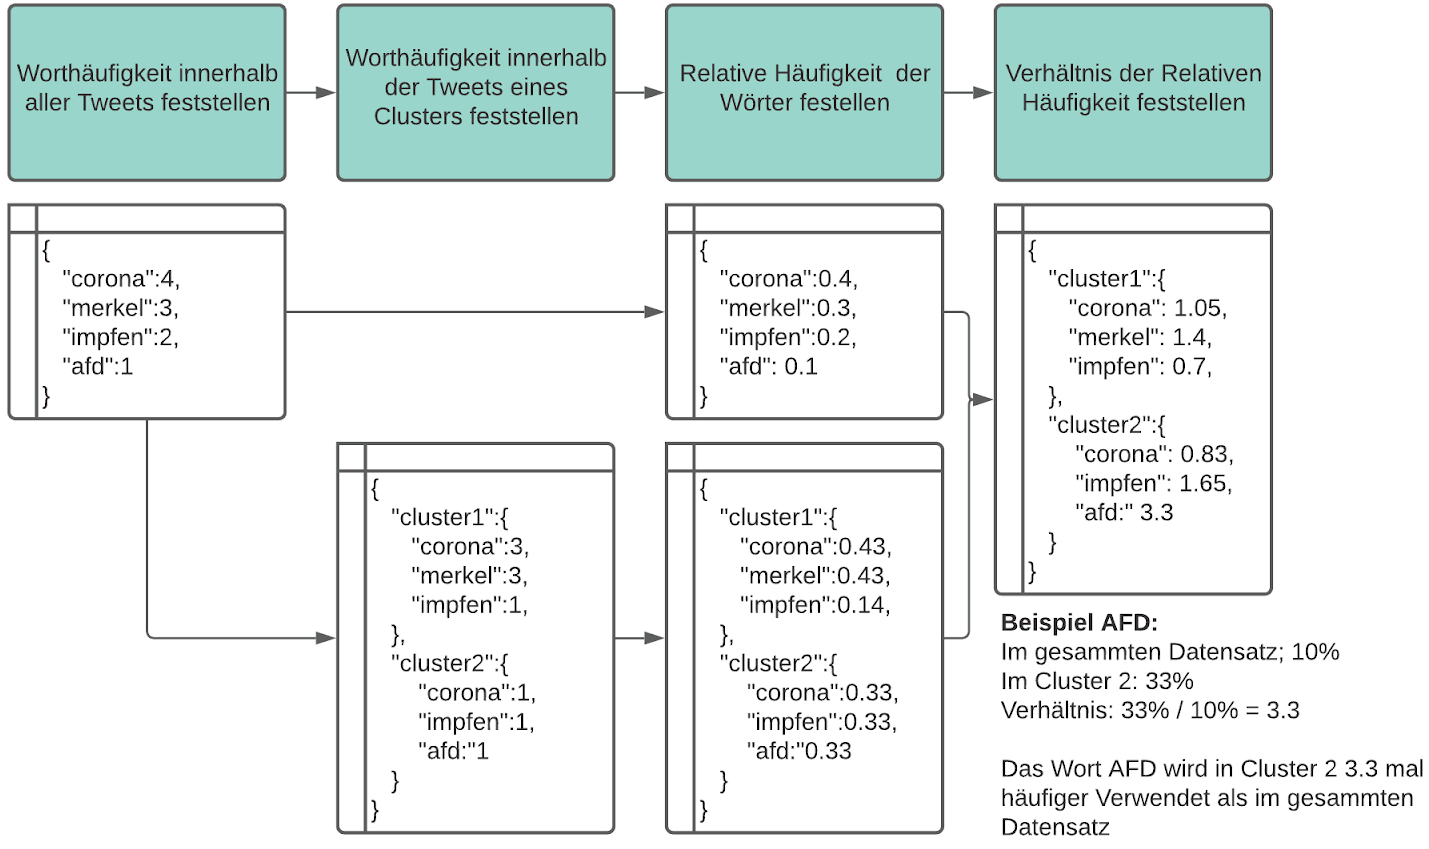
\includegraphics[width=\linewidth]{images/getting_cluster_topics}
	\caption{Bestimmung der Themen innerhalb der Cluster}
	\label{fig:prozess_topics}
\end{figure}





